\section{Design}
\label{sec:sidekick:design}

This section describes our design for a Sidekick protocol built around
quACKs. This includes the setup and configuration of a Sidekick
connection, how a data sender detects loss from a quACK, and a path-aware
modification to CUBIC called PACUBIC for congestion-controlled base
protocols.

%%%%%%%%%%%%%%%%%%%%%%%%%%%%%%%%%%%%%%%%%%%%%%%%%%%%%%%%%%%%%%%%%%%%%%%%%%%%%%%

\subsection{PEP discovery mechanism}
\label{sec:sidekick:design:discovery}

% In most settings, such as 4G/5G cellular networks,
PEPs have traditionally been deployed as transparent proxies, silently
interposing on end-to-end connections when they are on the network path.
Endpoints therefore need a way to detect
Sidekick proxies and inform them of where to send quACKs.  Because
of network address translation, all communication to the proxy must be
initiated by the endpoint or use the same IP addresses and port numbers of the
base connection.

Our design has endpoints signal Sidekick support by sending a
distinguished packet containing a 128-byte \texttt{sidekick-request} marker
along the base connection.
Such inline signaling could confuse hosts when only one endpoint supports Sidekick,
but this approach target protocols
such as QUIC that discard cryptographically unauthenticated data anyway.  It
would be cleaner to signal support through out-of-band UDP options~\cite
{ietf-tsvwg-udp-options-28}, which we may hope to do once standardized.
The proxy replies to a \texttt{sidekick-request} packet by sending a special packet from
the other endpoint's IP address and port number back to the original endpoint.
This packet
contains a \texttt{sidekick-reply} marker, an opaque session ID, and an IP
address and port number for communicating with the proxy.

% Sidekick connections can be configured explicitly or implicitly.
In systems that explicitly configure proxies, such as Apple's iCloud Private
Relay~\cite{icloud-private-relay} based on MASQUE~\cite
{kosek2021masque,kramer2021masquepep}, proxies can simply negotiate the Sidekick
connection during session establishment. However, any explicit proxy configuration
has the disadvantage that the proxy may not be on the most direct network path.
Explicit proxies also make mobility and handoffs more challenging.

\subsubsection{Security.}
A malicious third-party could execute a reflection amplification attack that
generates a large amount of traffic while hiding its source. This is
possible because the endpoint requests quACKs to a different port and (for some
carrier-grade NATs) IP address from the underlying session. To mitigate this,
each quACK can contain a quota, initially 1, of remaining quACKs the proxy
will send as well as an updated session ID\@.
The quota and session ID ensure only the endpoint can increase the quota or
otherwise reconfigure the session.

An adversarial PEP could send misleading information to the endpoint. Note that
only on-path PEPs can send credible information, since they refer to unique
packet identifiers.
To mitigate this, the endpoint can consider PEP feedback along with
end-to-end metrics to determine whether to keep using the PEP. The endpoint can
always opt out of the PEP and fall back to end-to-end mechanisms, and the PEP cannot actively manipulate traffic any
more than outside a Sidekick setting.

%%%%%%%%%%%%%%%%%%%%%%%%%%%%%%%%%%%%%%%%%%%%%%%%%%%%%%%%%%%%%%%%%%%%%%%%%%%%%%%

\subsection{Sidekick protocol messages}
\label{sec:sidekick:design:messages}

\begin{figure}[t]
    % \centering
    % Client payloads
    \begin{subfigure}[b]{0.48\linewidth}
        \begin{protopayload}{\texttt{Init}}
            \begin{lstlisting}[language=Rust]
epoch: u32;
base_conn: [u8; 12];
quack_ty: u8;
num_symbols: u8;
id_offset: u16;
quack_pkts: u16;
quack_ms: u16;
            \end{lstlisting}
        \end{protopayload}
        \begin{protopayload}{\texttt{Reset}}
            \begin{lstlisting}[language=Rust]
epoch: u32;
errno: u32;
            \end{lstlisting}
        \end{protopayload}
        \caption{Client payloads.}
        \label{fig:sidekick:payloads:client}
    \end{subfigure}
    \hfill
    % Proxy payloads
    \begin{subfigure}[b]{0.48\linewidth}
        \begin{protopayload}{\texttt{InitACK}}
            \begin{lstlisting}[language=Rust]
epoch: u32;
udp_port: u16;
errno: u32;
            \end{lstlisting}
        \end{protopayload}
        \begin{protopayload}{\texttt{QuACK}}
            \begin{lstlisting}[language=Rust]
count: u32;
last_element: u32;
code: Vec<Symbol>;
            \end{lstlisting}
        \end{protopayload}
        \caption{Proxy payloads.}
        \label{fig:sidekick:payloads:proxy}
    \end{subfigure}
  % Caption
  \caption{Sidekick protocol messages to configure and reset the Sidekick
  connection.}
  \label{fig:sidekick:payloads}
\end{figure}


Once the endpoint has an IP address and port for communicating with the proxy, it
can establish an adjacent Sidekick connection with the proxy from a different
local UDP port. The endpoint can then send various messages to the proxy to
configure the connection and reset bad state (\Cref{fig:sidekick:payloads:client}),
while receiving quACKs to decode and adjust the behavior of the base connection
(\Cref{fig:sidekick:payloads:proxy}).

\subsubsection{Configuration.}
In the \texttt{Init} message, the endpoint configures (i) which quACK construction
to use and the number of symbols, (ii) a byte offset into the packet payload at
which to compute the 4-byte identifier, and (iii) the interval at which the PEP
should send quACKs.
The proxy accepts or rejects these configurations with an \texttt{InitACK}
and, if accepted, immediately begins to send \texttt{QuACK} messages.

The number of symbols represents the upper bound on the number of missing
packets between quACKs, in practice the number of ``holes'' among the packets
that are selectively ACKed. This bound depends on the quACK interval, and
should be set based on how precise loss detection needs to be and other
link qualities. For example, the number of symbols should be larger to
detect congestive loss in the queue of a bottleneck link, or smaller to detect
transmission error on a lossy link.

The quACK interval is expressed in terms of time or number of packets,
 e.g., every $N$ milliseconds or every $N$ packets, as in a TCP delayed ACK.
The endpoint determines the desired interval based on its estimated
RTT of the base connection and its application objectives. For example, the
endpoint may want to receive quACKs more frequently for latency-sensitive
applications or lower-RTT paths.

\subsubsection{Resets.}
The Sidekick protocol allows the endpoint to tell the PEP to reinitialize the
quACK. The \texttt{Reset} message acts as a synchronization point in the base
connection in which both the endpoint and proxy disregard old packets and start
a new cumulative quACK. This is helpful if the quACK becomes invalid, such as
if the number of missing packets exceeds the maximum bound. It is always safe
to reset the quACK, or even to ignore the PEP entirely and fall back to the
base protocol's end-to-end mechanisms.

%%%%%%%%%%%%%%%%%%%%%%%%%%%%%%%%%%%%%%%%%%%%%%%%%%%%%%%%%%%%%%%%%%%%%%%%%%%%%%%
%%%%%%%%%%%%%%%%%%%%%%%%%%%%%%%%%%%%%%%%%%%%%%%%%%%%%%%%%%%%%%%%%%%%%%%%%%%%%%%
%%%%%%%%%%%%%%%%%%%%%%%%%%%%%%%%%%%%%%%%%%%%%%%%%%%%%%%%%%%%%%%%%%%%%%%%%%%%%%%

\subsection{Path-aware sender behavior enabled by the quACK}
\label{sec:sidekick:design:sender}

Now we discuss sender-side behaviors that are enabled by the
Sidekick protocol and which are helpful across several scenarios: detecting
packet loss from a decoded quACK, earlier retransmissions, and path-aware
congestion control to emulate the congestion response of a split TCP connection.

%%%%%%%%%%%%%%%%%%%%%%%%%%%%%%%%%%%%%%%%%%%%%%%%%%%%%%%%%%%%%%%%%%%%%%%%%%%%%%%

\subsubsection{Loss detection.}

The endpoint knows definitively which packets have been received by the proxy from
a decoded power sum quACK. Next, it must determine from the remaining packets which ones
have been dropped and which are still in-flight, including if there has been a
reordering of packets. In-flight packets are later classified as received or
dropped based on future quACKs.

When there is no reordering, the packets that are dropped are just the ``holes''
among the packets that are selectively ACKed by the quACK. In particular, these
are the holes when considering sent packets in the order they were sent up to
the last element received, which represents the last selective ACK. To identify
these dropped packets, the endpoint encodes $t$ cumulative power sums of its sent
packets up to the last element received. The difference between these power
sums and the power sums in the quACK represents the dropped packets. The endpoint
``removes'' the identifiers of dropped packets from its cumulative power sums,
ensuring that the only packets that contribute to the threshold limit are those
that went missing since decoding the last quACK.

To account for reordering in loss detection, our design has the Sidekick
protocol use an
algorithm similar to the 3-duplicate ACK rule in
TCP~\cite{rfc5681tcp,rfc2001tcp}. In TCP, if three or more duplicate ACKs are
received in a row, it is a strong indication that a segment has been lost. Our
design similarly considers a packet lost only if three or more packets sent
after the missing packet have been received. Other mechanisms could involve
timeouts for individual packets similar to the RACK-TLP loss detection
algorithm for TCP~\cite{rfc8985}.

\subsubsection{Earlier retransmissions.}

On detecting loss, a data sender can immediately retransmit missing packets.
Assuming reliability is a desired property of the base protocol, this allows
the data sender to retransmit the packet earlier than if it had waited for an
end-to-end ACK.

%%%%%%%%%%%%%%%%%%%%%%%%%%%%%%%%%%%%%%%%%%%%%%%%%%%%%%%%%%%%%%%%%%%%%%%%%%%%%%%

\subsubsection{Path-aware congestion control.}

The congestion response of a congestion-controlled base protocol to lost packets
that they retransmit due to quACKs determines whether the connection achieves
any throughput improvements. Consider what happens if the base protocol treats
loss detected from quACKs the same as from end-to-end ACKs. Since loss is a
binary signal in ``loss-based'' congestion control algorithms such as
CUBIC~\cite{ha2008cubic}, the connection would have the same, low throughput as
an end-to-end connection. If the base protocol had no congestion response at
all, it would not be fair to connections without Sidekick assistance, and in
the worst case, retransmissions from quACKs could cause congestion collapse.

Thus congestion-controlled base protocols must have some congestion response to
loss from quACKs to ensure friendliness with existing congestion control
schemes that do consider the loss. Our benchmark for a fair response is to
achieve the same throughput as TCP CUBIC in the presence of a
connection-splitting TCP PEP in the same settings. We refer to CUBIC with a
split connection as ``split CUBIC'', which has distinct behavior from
``end-to-end CUBIC'' without a connection-splitter and has notably higher
throughput. However, a path-aware congestion response can only change the
behavior at the endpoint, since packets are opaque to the proxy, in order to
emulate the split congestion-control behavior of split CUBIC. We describe
the algorithmic details of in \Cref{sec:sidekick:pacubic}.

\section{Path-aware CUBIC congestion control}
\label{sec:sidekick:pacubic}

Here, we propose PACUBIC, or path-aware CUBIC, an algorithm that emulates
``split CUBIC'' behavior. PACUBIC uses knowledge of where loss occurs along a
network path to improve connection
throughput compared to end-to-end CUBIC, while remaining fair to competing flows.

\subsection{Background: CUBIC}

Recall that CUBIC~\cite{ha2008cubic} reduces its congestion window by a
multiplicative decrease factor,
$\beta = \beta^* = 0.7$, when observing loss (a congestion event), and otherwise
increases its window based on a real-time dependent cubic function with scaling
factor $C=C^*=0.4$:
\[
cwnd = C(T-K)^3 + w_{max} \text{ where } K = \sqrt[3]{\frac{w_{max}(1-\beta)}{C}}.
\]

\noindent Here, $cwnd$ is the current congestion window,
$w_{max}$ is the window size just before the last reduction,
and $T$ is the time elapsed since the last window reduction.

\subsection{PACUBIC algorithm}

While a split CUBIC connection has \emph{two} congestion windows,
end-to-end PACUBIC only has \emph{one} window representing the in-flight bytes
of the end-to-end connection.
Conceptually, we want an algorithm that enables PACUBIC's single
congestion window to match the sum of the split connection's two congestion
windows.

PACUBIC effectively makes it so that we reduce and grow $cwnd$
proportionally to the number of in-flight bytes on the path segment
of where the last congestion event occurred.
Let $r$ be the estimated ratio of the RTT of the near path segment
(between the data sender and the proxy) to the RTT of the entire connection
(between end hosts).
We use $r$ as a proxy for the ratio of the number of in-flight bytes. If the
last congestion event came from a quACK, we use the same real-time dependent
cubic function but with the following constants:
\[
\beta = 1 - r(1-\beta^*)\text{ and }C = \frac{C^*}{r^3}.
\]
\noindent If the last congestion event came from an end-to-end ACK, then we use
the original $\beta$ and $C$.

While this algorithm resembles the congestion behavior of split CUBIC, it is
simply an approximation. PACUBIC does not know the exact number of bytes
in-flight on each path segment, and the sum of the two congestion windows is
simply a heuristic for an inherently different split connection. The main
takeaway is that knowing where loss occurs can inform congestion control. We
generally hope that quACKs can lead to the development of smarter, path-aware
congestion-control schemes.

\subsection{Intuitive correctness analysis}
\label{sec:sidekick:pacubic:analysis}

\begin{figure}[t]
\centering
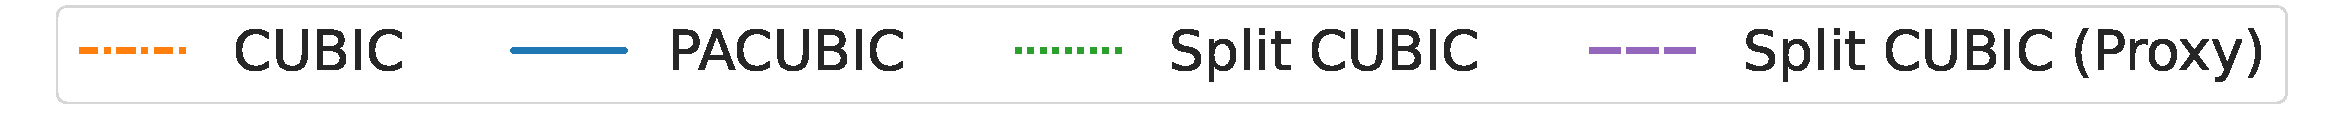
\includegraphics[width=0.8\linewidth]{sidekick/figures/cwnd_legend.pdf}\\
\begin{subfigure}{0.32\linewidth}
  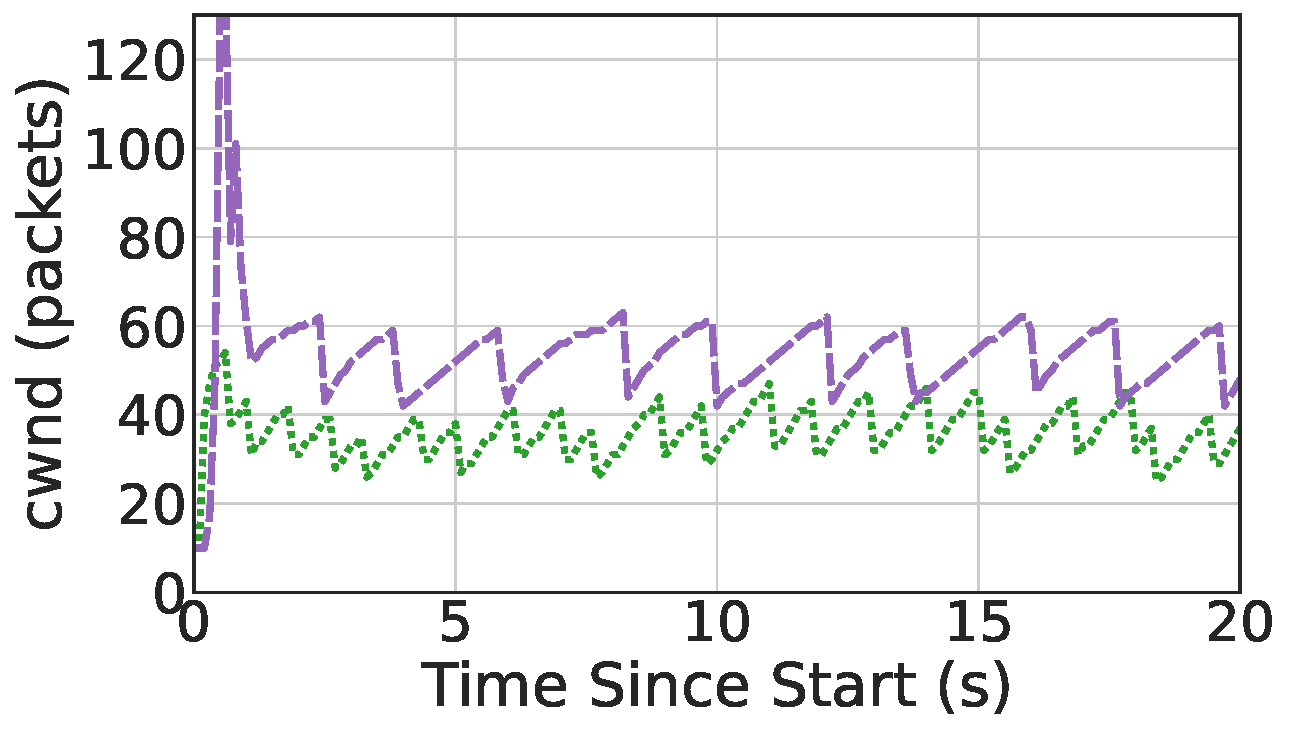
\includegraphics[width=\linewidth]{sidekick/figures/cwnd_split_loss0p.pdf}
  \caption{Split CUBIC, 0\% loss.}
  \label{fig:sidekick:pacubic:split-loss0p}
\end{subfigure}
\begin{subfigure}{0.32\linewidth}
  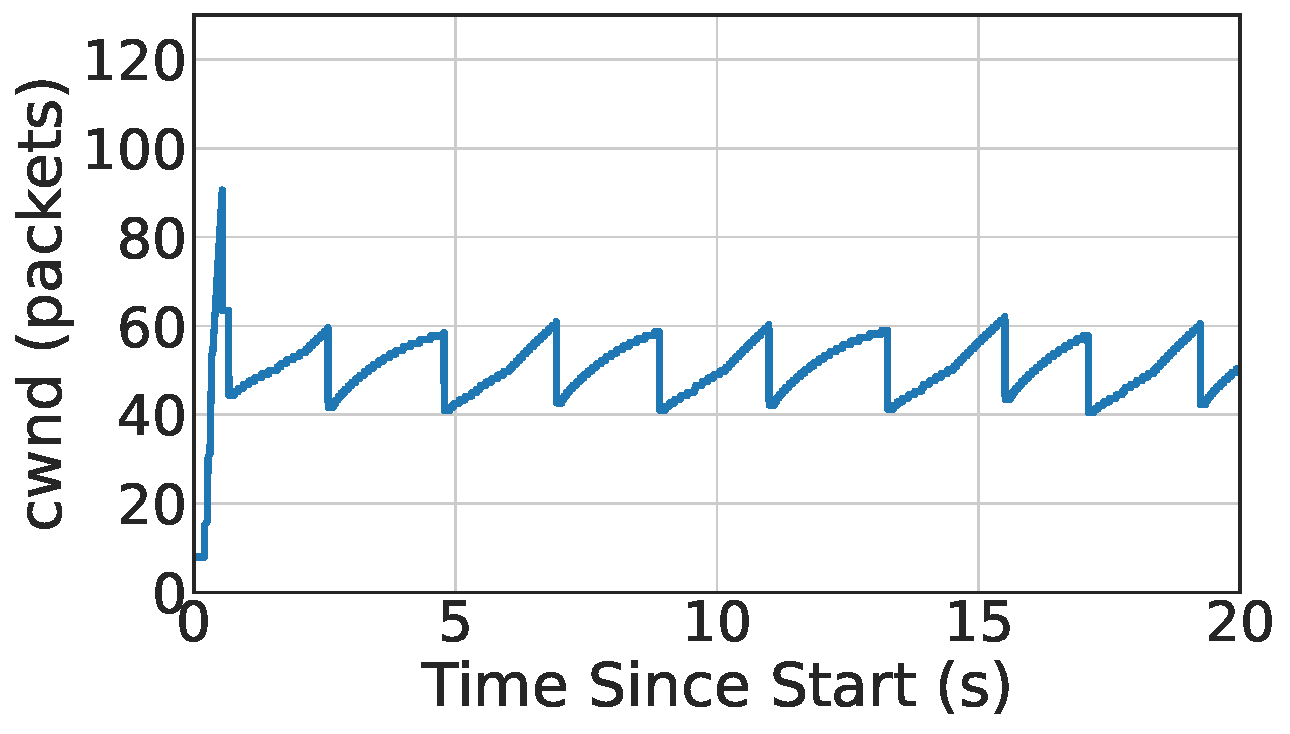
\includegraphics[width=\linewidth]{sidekick/figures/cwnd_pacubic_loss0p.pdf}
  \caption{PACUBIC, 0\% loss.}
  \label{fig:sidekick:pacubic:pacubic-loss0p}
\end{subfigure}
\begin{subfigure}{0.32\linewidth}
  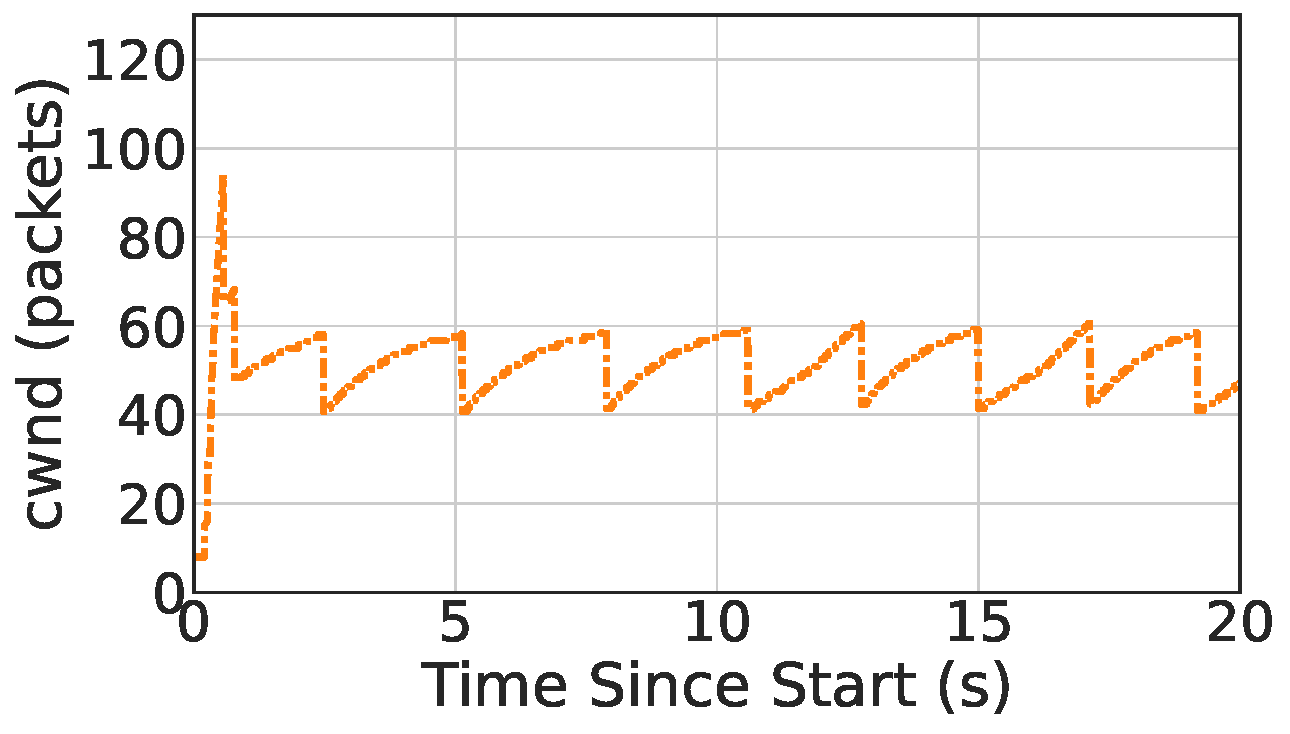
\includegraphics[width=\linewidth]{sidekick/figures/cwnd_cubic_loss0p.pdf}
  \caption{CUBIC, 0\% loss.}
  \label{fig:sidekick:pacubic:cubic-loss0p}
\end{subfigure}
\begin{subfigure}{0.32\linewidth}
  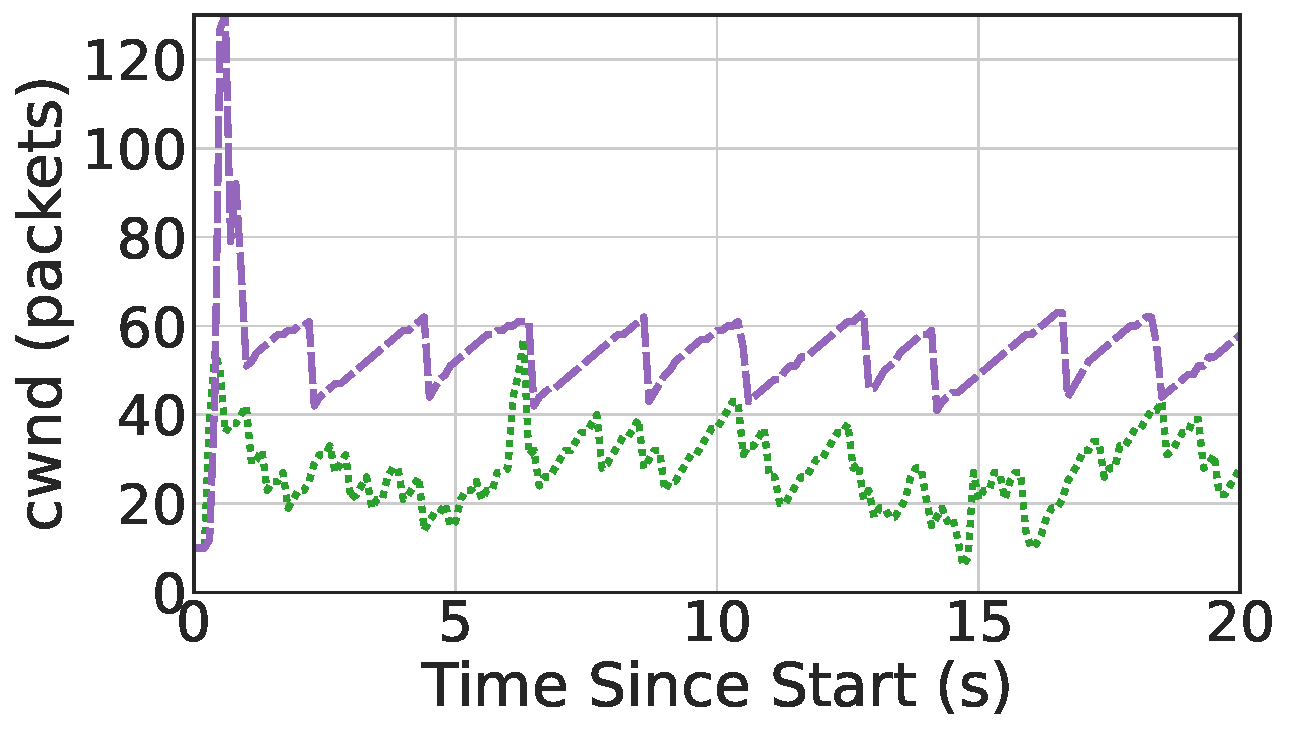
\includegraphics[width=\linewidth]{sidekick/figures/cwnd_split_loss1p.pdf}
  \caption{Split CUBIC, 1\% loss.}
  \label{fig:sidekick:pacubic:split-loss1p}
\end{subfigure}
\begin{subfigure}{0.32\linewidth}
  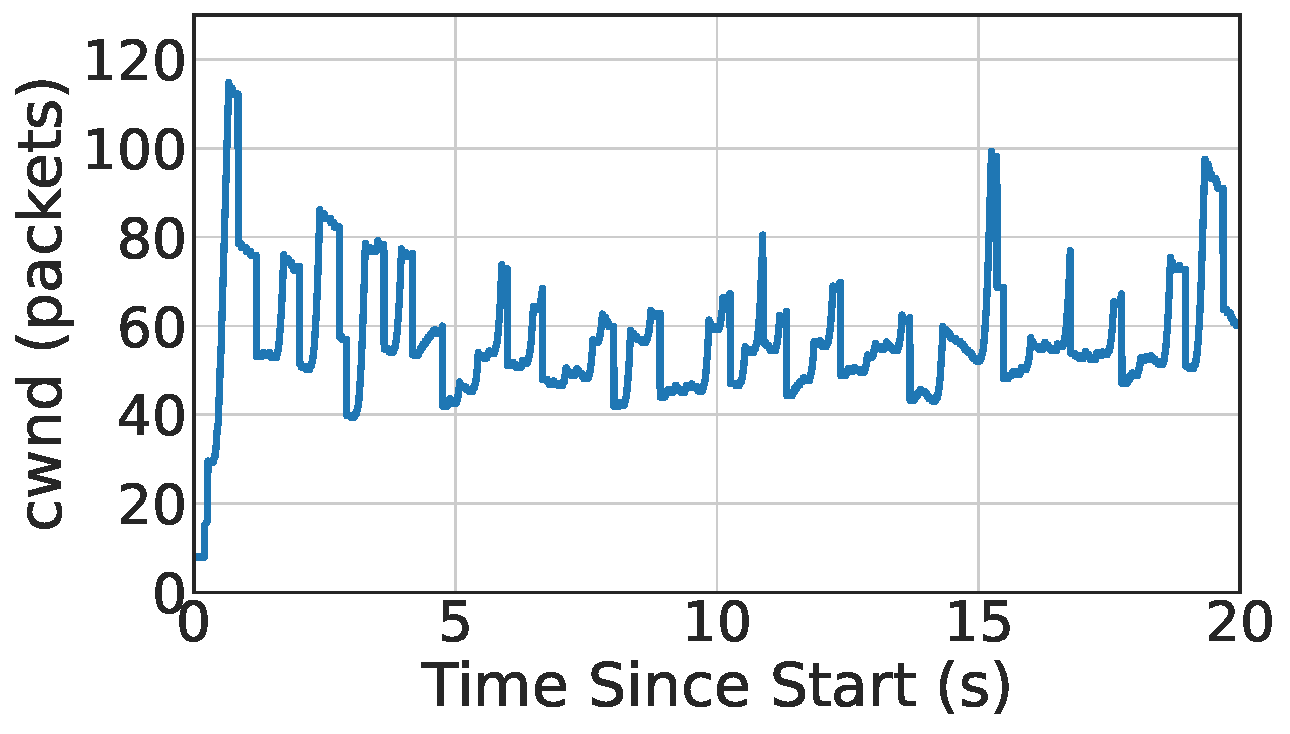
\includegraphics[width=\linewidth]{sidekick/figures/cwnd_pacubic_loss1p.pdf}
  \caption{PACUBIC, 1\% loss.}
  \label{fig:sidekick:pacubic:pacubic-loss1p}
\end{subfigure}
\begin{subfigure}{0.32\linewidth}
  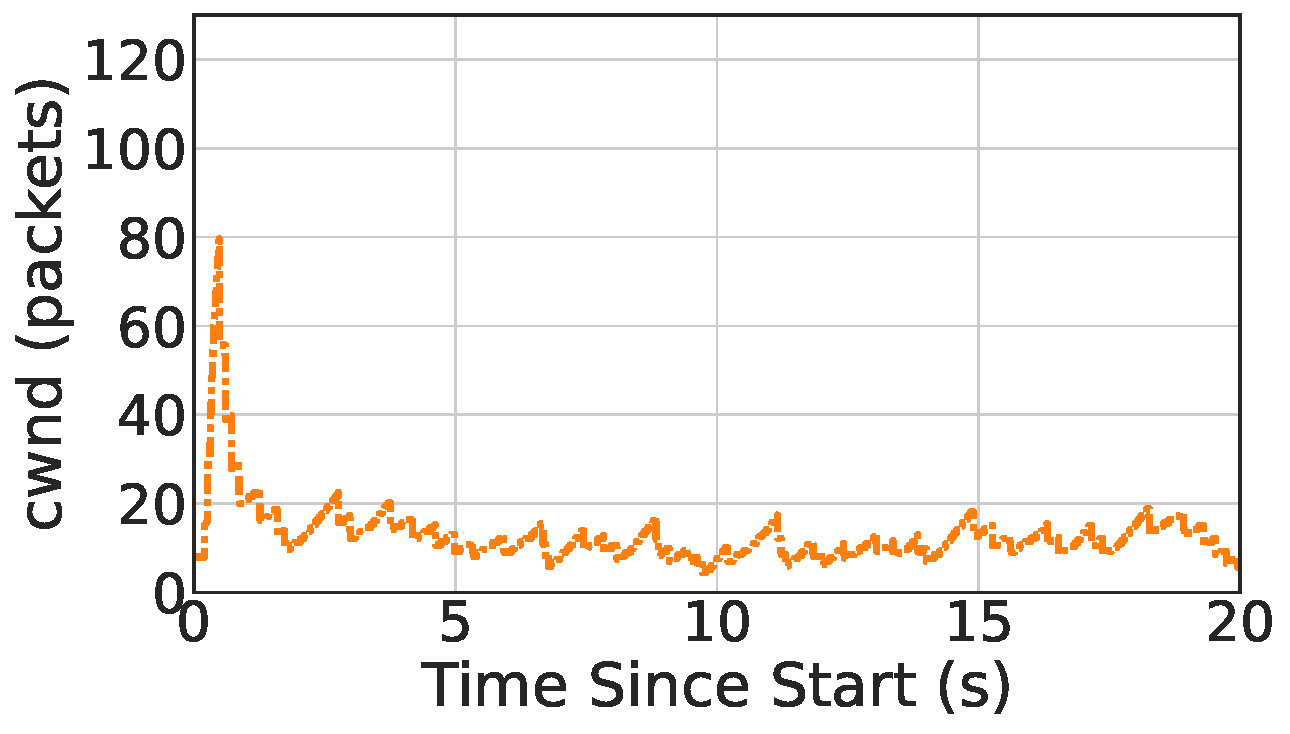
\includegraphics[width=\linewidth]{sidekick/figures/cwnd_cubic_loss1p.pdf}
  \caption{CUBIC, 1\% loss.}
  \label{fig:sidekick:pacubic:cubic-loss1p}
\end{subfigure}
\caption{Congestion window of a long-running upload in Scenario \#2
(\Cref{tab:sidekick:experimental-scenarios}) with $0\%$ and $1\%$ loss on the
near path segment. The cwnd is measured at the data sender,
except for split CUBIC whose split connection also has a cwnd at the proxy.
PACUBIC reacts to every congestion event while keeping the cwnd high.
CUBIC performs poorly when there is loss on the near path segment.
CUBIC and PACUBIC are implemented in QUIC, while split CUBIC is implemented
in TCP using a PEP.
}
\label{fig:sidekick:pacubic}
\end{figure}


Here, we dive deeper into the intuition behind the PACUBIC constants $\beta$
and $C$, including how they were derived and why
the PACUBIC algorithm achieves similar congestion behavior to split CUBIC.

\subsubsection{Analysis.}

Consider the same network topology as \Cref{fig:sidekick:overview} in which a
data sender uploads a large file to a data receiver, with help from a Sidekick
proxy in the middle of the connection. The near path segment connects the data sender
to the proxy, and the far path segment connects the proxy to the data receiver.
The near path segment is low-delay with varying random loss, and the far path segment is
high-delay with no random loss. The far path segment is the bottleneck link in terms
of bandwidth.
The actual link parameters are the same as in Scenario \#2 of
\Cref{tab:sidekick:experimental-scenarios}.

To conceptually motivate PACUBIC, let's first discuss how split CUBIC would
behave in this setting.
Consider the congestion windows of each half of the split
connection, one taken at the data sender and one at the proxy
(\Cref{fig:sidekick:pacubic:split-loss0p,fig:sidekick:pacubic:split-loss1p}). The far path
segment experiences only congestive loss, leading the window at the proxy to
fluctuate around the segment's bandwidth-delay product regardless of the loss on the near path
segment. The window at the data sender independently determines whether the
packets that reach the proxy will be able to fully utilize the window set at
the far path segment. We will see that the data sender is able to achieve this at low random
loss rates, but becomes the bottleneck as loss rates increase
(\Cref{fig:sidekick:fairness-line}).

While split CUBIC has two windows, PACUBIC only has one
window representing the in-flight bytes of the end-to-end connection.
PACUBIC considers loss detected from both quACKs and end-to-end ACKs.
Conceptually, we want an algorithm that would enable PACUBIC's single
congestion window to match the sum of CUBIC's two congestion windows, or
the total number of in-flight bytes.
% That is the motivation behind adjusting the window proportionally to the
% number of in-flight bytes on each path segment, depending on where the loss
% occurred.

With no random loss on the near path segment, PACUBIC
(\Cref{fig:sidekick:pacubic:pacubic-loss0p}) behaves the same as end-to-end CUBIC
(\Cref{fig:sidekick:pacubic:cubic-loss0p}). The congestion window is entirely governed
by end-to-end ACKs since the far path segment is the bottleneck link. Note that
while the sender may be able to deduce that a loss occurred on the far path
segment by combining info from the quACK with the end-to-end ACK, PACUBIC
conservatively treats the loss as occurring anywhere on the path.

With some random loss on the near path segment, PACUBIC grows and reduces $cwnd$
based on where the last congestion event occurs
(\Cref{fig:sidekick:pacubic:pacubic-loss1p}). Note that if the congestion window $cwnd$
represents the bytes in-flight in the end-to-end connection, then $r \cdot cwnd$
represents the proportion of bytes in-flight on the near path segment. At a
high level, if the data sender discovers loss on the near path segment via the
quACK, it holds the $(1-r)\cdot cwnd$ portion of the ``far window'' constant
while applying the CUBIC algorithm to the remaining $r \cdot w_{max}$ of the
``near window'', representing the bottleneck link.

Mathematically, instead of reducing $w_{max}$, the window size just before the
last reduction, by $(1-\beta^*) \cdot w_{max}$, PACUBIC reduces it by only
$[1 - (1-r(1-\beta^*))] \cdot w_{max} = r(1-\beta^*) \cdot w_{max}$.
That is $r$ times the original reduction, a \emph{smaller} amount.
We use the RTT ratio $r$ (near path segment to end-to-end)
% indicating the RTT ratio of near path segment vs.~far path segment)
as a proxy for the ratio of the number of in-flight bytes.

Similarly, instead of using a cubic growth function with scaling factor $C^*$
and inflection point $K = K^* = \sqrt[3]{w_{max}(1-\beta^*)/C^*}$,
we use a larger scaling factor $C = C^*/r^3$
and thus a shorter inflection point:
\[
K = \sqrt[3]{\frac{w_{max}(1-\beta)}{C}}
= \sqrt[3]{\frac{r\cdot w_{max}(1-\beta^*)}{C^* / r^3}}
= r^{4/3} \cdot K^*.
\]
The shorter inflection point leads the congestion window to \emph{grow more
quickly} since the sender also reacts to feedback about loss more quickly over
the low-delay link.
% Since similarly proportional to $w_{max}$, so with $C'$, we both reduce the
% inflection point $K$ and the growth rate $C$ of the function proportionally to
% the number of bytes in-flight on the near path segment.

At times, there can be loss detected both in quACKs and in end-to-end ACKs.
The end-to-end ACKs have a greater effect since they reduce the congestion
window by a larger proportion, until the remaining path segment with loss is the
bottleneck link. In this scenario with loss, the bottleneck link at equilibrium
is the near path segment.
At this point, the quACK primarily determines the congestion window updates. If
the far path segment were to become the bottleneck again, the data sender would
detect a congestion event via the end-to-end ACK.

\subsubsection{Limitations.}

PACUBIC has several limitations. Although it beats end-to-end CUBIC, we will see
that it still performs worse than split CUBIC, especially at high loss rates
(\Cref{fig:sidekick:fairness-line}). Also, it doesn't consider loss on the far
path segment any differently than end-to-end CUBIC, unlike split CUBIC which
treats the two split connections independently. PACUBIC emulates the congestion
control behavior and fairness of split CUBIC fairly well as a heuristic, but
would benefit from an analysis in a wider variety of network scenarios. It
would also benefit from a side-by-side fairness comparison against congestion
control algorithms such as BBR~\cite{cardwell2024bbr-ietf-draft} that perform
well in the same scenarios. We'd like a takeaway of PACUBIC to be that knowing
where loss occurs can cleverly inform congestion control.
